%!TEX root = ..\..\main.tex
\chapter{The Coupling Time on the Cycle}
\label{Ch:1D}

\lhead{Chapter \ref{Ch:1D}. \emph{The Coupling Time on the Cycle}}

	In this chapter we consider the Ising heat-bath Glauber dynamics (as described in Section \ref{sec:heat-bath glauber dynamics definition}) on the cycle $G_n = (\mathbb{Z}/n\mathbb{Z})$. The object of interest is the coupling time, $T_n$, which was defined in Section \ref{sec:the coupling time}. To simplify the analysis we study another random variable, defined in Section \ref{sec:information percolation on the cycle}, which has the same distribution as $T_n$. The main result is Theorem \ref{thm:Coupling Distribution on Cycle} which establishes that $T_n$ converges in distribution to a Gumbel distribution at all temperatures. This confirms, for $d = 1$, a conjecture by \citeauthor{Collevecchio2018-nq} that the coupling time of the Ising heat-bath process on the lattice $G_L = (\mathbb{Z}/L\mathbb{Z})^d$ converges to a Gumbel distribution as $L \rightarrow \infty$ for all $\beta < \beta_\mathrm{c}$ \cite[Conjecture 7.1]{Collevecchio2018-nq} (We treat higher dimensions, and more generally any vertex transitive graphs, in Chapter \ref{Ch:GeneralResults}). Of course, in one dimension, all temperatures are part of the high temperature regime \cite{Friedli2017-xm}, and our result holds for any inverse-temperature $\beta$.

	There is some intuition behind why we might expect that the coupling time converges to a Gumbel distribution. It is based on the belief that when the temperature is in the high-temperature regime, the dynamics behave qualitatively as if $\beta = 0$. In the $\beta = 0$ case, the spins update independently of their neighbours, and thus the top and bottom chains can be coupled so that they agree on each vertex that has been updated. The coupling time is then precisely the time it takes for each vertex to be updated. This corresponds to the coupon collector's problem, which is known to have a Gumbel limit \cite{Erdos1961-ti}.

	As mentioned in Section \ref{sec:summary of CFTP}, the coupling time is of practical interest since its distribution is the same as that of the running time of the coupling from the past (CFTP) algorithm. Our result shows that when running the Glauber heat-bath dynamics for the Ising model on a large enough cycle, the running time of CFTP can be approximated by a Gumbel distribution. We note that even though one is typically more interested in the Ising model on lattices of dimension at least two (so that there exists a phase transition), the one dimensional case proves to be a useful test case for the proof techniques. Furthermore, the applicability of Theorem \ref{thm:Coupling Distribution on Cycle} to the full high temperature regime justifies a treatment separate to that of the higher dimensional case considered in Chapter \ref{Ch:GeneralResults}, the proof of which holds only for sufficiently high temperatures.

	% [WHAT IT MEANS]

	% [WHATS THE POINT?]

	\begin{theorem}
	\label{thm:Coupling Distribution on Cycle}
		Let $T_n$ be the coupling time for the continuous-time Ising heat-bath Glauber dynamics for the zero-field ferromagnetic Ising model on the cycle $(\mathbb{Z} / n\mathbb{Z})$. Then for any inverse-temperature $\beta$, there exists a subsequence $(T_m)$ of $(T_n)$ such that
		\begin{equation}
			\lim_{m \rightarrow \infty} \prob\left[T_m < \frac{z + \ln m}{\theta}\right] = \euler^{-C_\theta \euler^{-z}}
		\end{equation}
		where $\theta = 1 - \tanh(2\beta)$ and $C_\theta$ is a positive constant satisfying
		\begin{equation}
			\frac{1}{2\sqrt{\frac{4}{\theta} - 1} - 1} \leq C_\theta \leq 1.
		\end{equation}
	\end{theorem}

	The proof of Theorem \ref{thm:Coupling Distribution on Cycle} will be given in Section \ref{sec:proof thm coupling cycle} after the essential preliminaries are presented. In Section \ref{sec:information percolation on the cycle} we describe some modified dynamics and show that the coupling time we construct from these has the same distribution as the coupling time defined in Section \ref{sec:the coupling time}. Then in Section \ref{sec:1D problem setup} we outline the overall approach to the proof and define some essential quantities. Finally, Section \ref{sec:additional lemmas 1D} contains additional lemmas that are used in Section \ref{sec:proof thm coupling cycle}.

	\section{A new coupling on the cycle}
	\label{sec:information percolation on the cycle}
	% On the cycle, the heat-bath dynamics allow for a new set of updates rules, to replace those from \eqref{eq:plusorminusrules}. The changed update rules provide another construction for the coupling of $\mathscr{T}_t$ and $\mathscr{B}_t$ but preserve the distribution of the coupling time, $T_n$. We use these new update rules because they result in much simpler update histories.

	On the cycle, we will use a different coupling of $\mathscr{T}_t$ and $\mathscr{B}_t$ via a new random mapping representation that will replace the update rule in \eqref{eq:plusorminusrules}. The new update rules simplify our update histories greatly by ensuring that each of the update histories never contain more than one vertex at any one time. However, we must be cautious. The coupling time is not just a property of the heat-bath dynamics, but also of the specific coupling we chose. Hence, we first verify that switching to our new rules does not change the distribution of $T_n$. 

	The new update rules are defined by using almost the same construction as in Section \ref{sec:the coupling time}. The one difference is that we replace \eqref{eq:plusorminusrules} as follows. When vertex $i$ updates, instead of comparing $U$ to the probability $p_i(\sigma)$ to determine the new spin, we instead chose a new spin $\sigma_i'$ via
	% state that when vertex $i$ updates, a spin $\sigma_i'$ is chosen via
	\begin{equation}
	\label{eq:new update rules}
		\sigma_i' = \begin{cases}
			+1 & U < \theta/2,\\
			\sigma_{i-1} & \theta/2 \leq U < 1/2,\\
			\sigma_{i+1} & 1/2 \leq U < 1 - \theta/2,\\
			-1 & U \geq 1 - \theta/2.
		\end{cases}
	\end{equation}
	where $U \in [0,1]$ is an independent uniform random variable as before. It is easy to see that these update rules give rise to the same transition rates as those in \eqref{eq:plusorminusrules}. To show that the coupling time is unchanged, it is sufficient to verify that the joint jump probabilities of $(\mathscr{T}_t[i], \mathscr{B}_t[i])$ are unchanged for each possible configuration of spins of vertices $i-1$ and $i+1$. There are only nine possible configurations for the two neighbours of $i$ in the top and bottom chain since $\mathscr{B}_t[i] \leq \mathscr{T}_t[i], \forall t$. Likewise, there are only three possible configurations for the updated spins $(\mathscr{T}_t[i]', \mathscr{B}_t[i]')$. Hence, given vertex $i$ updates at time $t$, we can easily calculate all the required jump probabilities as shown in Table \ref{tab: joint jump probs}. These are unchanged whether using \eqref{eq:plusorminusrules} or \eqref{eq:new update rules} and so the new rules do not change the coupled dynamics.

	[MAKE INTO LEMMA?]

	\begin{table}
	\begin{tabular}{c || c c c}
	\diagbox[]{		
		\begin{tabular}{@{}c@{}}
		$\mathscr{T}_t = \cdot$ \\ 
		$\mathscr{B}_t = \cdot$ 
		\end{tabular}
	}{
		$\prob[(\mathscr{T}_t[i]', \mathscr{B}_t[i]') = \cdot \,]$
	}
	&(1,1)&(1,-1)&(-1,-1)\\
	\hline
	\hline
		\begin{tabular}{@{}c@{}}
		$(\dots, 1, \mathscr{T}_t[i], 1,\dots)$ \\ 
		$(\dots, 1, \mathscr{B}_t[i], 1,\dots)$ 
		\end{tabular}
	&$1 - \theta$& 0 & $\frac{\theta}{2}$\\
	\hline
		\begin{tabular}{@{}c@{}}
		$(\dots, 1, \mathscr{T}_t[i], 1,\dots)$ \\ 
		$(\dots, 1, \mathscr{B}_t[i], -1,\dots)$ 
		\end{tabular}
	&$\frac{1}{2}$& $\frac{1-\theta}{2}$ & $\frac{\theta}{2}$\\
	\hline
		\begin{tabular}{@{}c@{}}
		$(\dots, 1, \mathscr{T}_t[i], 1,\dots)$ \\ 
		$(\dots, -1, \mathscr{B}_t[i], 1,\dots)$ 
		\end{tabular}
	&$\frac{1}{2}$& $\frac{1-\theta}{2}$ & $\frac{\theta}{2}$\\
	\hline
		\begin{tabular}{@{}c@{}}
		$(\dots, 1, \mathscr{T}_t[i], 1,\dots)$ \\ 
		$(\dots, -1, \mathscr{B}_t[i], -1,\dots)$ 
		\end{tabular}
	& $\frac{\theta}{2}$ & $1 - \theta$ & $\frac{\theta}{2}$ \\
	\hline
		\begin{tabular}{@{}c@{}}
		$(\dots, 1, \mathscr{T}_t[i], -1,\dots)$ \\ 
		$(\dots, 1, \mathscr{B}_t[i], -1,\dots)$ 
		\end{tabular}
	& $\frac{1}{2}$ & 0 & $\frac{1}{2}$ \\
	\hline
		\begin{tabular}{@{}c@{}}
		$(\dots, 1, \mathscr{T}_t[i], -1,\dots)$ \\ 
		$(\dots, -1, \mathscr{B}_t[i], -1,\dots)$ 
		\end{tabular}
	& $\frac{\theta}{2}$ & $\frac{1-\theta}{2}$ & $\frac{1}{2}$ \\
	\hline
		\begin{tabular}{@{}c@{}}
		$(\dots, -1, \mathscr{T}_t[i], 1,\dots)$ \\ 
		$(\dots, -1, \mathscr{B}_t[i], 1,\dots)$ 
		\end{tabular}
	& $\frac{1}{2}$ & 0 & $\frac{1}{2}$ \\
	\hline
		\begin{tabular}{@{}c@{}}
		$(\dots, -1, \mathscr{T}_t[i], 1,\dots)$ \\ 
		$(\dots, -1, \mathscr{B}_t[i], -1,\dots)$ 
		\end{tabular}
	& $\frac{\theta}{2}$ & $\frac{1-\theta}{2}$ & $\frac{1}{2}$ \\
	\hline
		\begin{tabular}{@{}c@{}}
		$(\dots, -1, \mathscr{T}_t[i], -1,\dots)$ \\ 
		$(\dots, -1, \mathscr{B}_t[i], -1,\dots)$ 
		\end{tabular}
	& $\frac{\theta}{2}$ & 0 & $1 - \theta$
	\end{tabular}
	\caption{Probabilities of updating from $(\mathscr{T}_t, \mathscr{B}_t)$ to $(\mathscr{T}_t', \mathscr{B}_t')$ given vertex $i$ updates at time $t$.}
	\label{tab: joint jump probs}
	\end{table}
	% It is easy to verify that for each possible configuration, the joint distribution for $\sigma_i'$ in the top and bottom chains is the same whether we use these rules or the ones given in \eqref{eq:plusorminusrules}. Hence the coupling time is unchanged in distribution in this new random mapping representation.

	\subsection{Update histories on the cycle}
	\label{sec:update histories on the cycle}
	Under the update rules in \eqref{eq:new update rules}, each time a vertex is updated, it is either an oblivious update with probability $\theta$, or it takes the spin of a uniformly chosen neighbour. Unlike the histories considered earlier (for example Figure \ref{fig:example percolation construction oblivious}), this time a non-oblivious update does not cause the history to branch out to both its neighbours. Rather, given a non-oblivious update to some vertex $v$, we only need to know the spins of one of its neighbours to update it (the left spin if $U  < 1/2$ and the right if $U \geq 1/2$). So the history simply moves either right or left without branching. As before, encountering an oblivious update causes $\mathcal{H}_i$ to terminate. 

	Let us give an explicit construction for the update histories just described. Let $N_t$ be the rate $n$ Poisson process used to continuize the discrete process and let $(\mathcal{V}_k, U_k)_{k\geq1}$ be the discrete noise sequence (as in Section \ref{sec:the coupling time}). For each vertex $i \in V$ define the thinned processes,
	\begin{align}
		K^i_t &= \#\{k \leq N_t: \mathcal{V}_k = i, U_k \in \left[0, \theta/2\right) \cup \left(1 - \theta/2, 1\right]\}\\
		L^i_t &= \#\{k \leq N_t: \mathcal{V}_k = i, U_k \in \left[\theta/2, 1/2\right)\}\\
		R^i_t &= \#\{k \leq N_t: \mathcal{V}_k = i, U_k \in \left[1/2, 1 - \theta/2\right)\}.
	\end{align}
	The process $K_t^i$ is Poisson with rate $\theta$ and gives the times when vertex $i$ has an oblivious update. The processes $L_t^i$ and $R_t^i$ are Poisson with rate $(1 - \theta)/2$ and give the times when $\sigma_i$ is replaced by $\sigma_{i-1}$ and $\sigma_{i+1}$ respectively.

	The collection of $K_i^t$, $L_t^i$ and $R_t^i$ for every $i \in V$ forms an encoding of the update sequence and may be represented graphically as follows. Place an $\times$ at every $(i, K_t^i) \in V \times [0, t_*]$. Draw a directed edge $(i, L_t^i) \rightarrow (v - 1, L_t^i)$ for every $L_t^i$ and draw a directed edge $(i, R_t^i) \rightarrow (v + 1, R_t^i)$ for every $R_t^i$. To construct the update histories, trace back in time from $t_*$ from each vertex, making turns along directed horizontal edges, and killing the process at any $\times$. An example of this graphical representation along with the update histories is shown in Figure \ref{fig:example histories 1D thinned poisson}.

	["SHOULD PROBABLY COMMENT ON WHY, IE WHY THEY HAVE THE RIGHT DISTRIBUTION"]

	[POINT OUT THIS IS SAME AS GRAPHICAL REPRESENTATION OF NOISY VOTER MODEL]
	% An example history using these new rules is shown in Figure \ref{fig:example percolation construction rightleft}. In a similar vein to Figures \ref{fig:example percolation construction oblivious} and \ref{fig:nonoblivious shrink} we represent each update $(\mathcal{V}, U, t)$ in the update sequence by placing at $(\mathcal{V}, t)$ one of the symbols $+$, $r$, $l$, or $-$ chosen according to $U$. We then trace back from time $t_*$, moving left or right when we encounter a $l$ or $r$ respectively, and terminating whenever we encounter a $+$ or $-$.

	% \begin{figure}
	% 	\centering
	% 	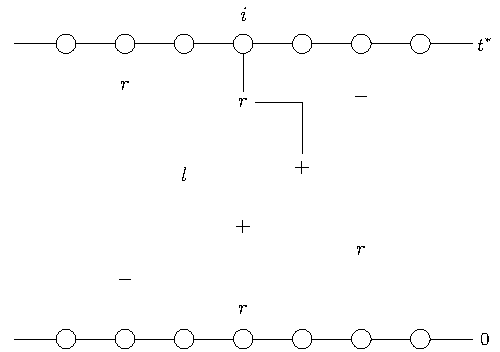
\includegraphics[width = 0.8\textwidth]{Figures/IsingCouplingTime/example_percolation_construction_rightleft.pdf}
	% 	\caption[The update sequence for a section of the cycle and the corresponding update history from vertex i using the new update rules.]{The update sequence for a section of the cycle and the corresponding update history from vertex $i$ using the new update rules. Vertex $i$ takes the same spin as the spin it terminates at, in this case $+1$.}
	% 	\label{fig:example percolation construction rightleft}
	% \end{figure}

	\begin{figure}
		\centering
		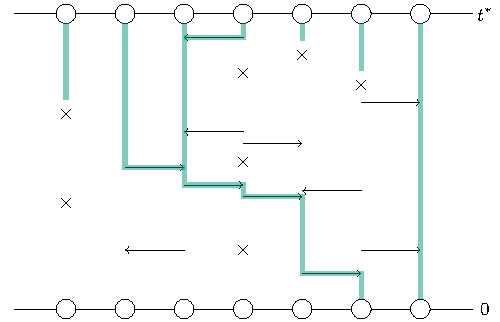
\includegraphics[width = 0.8\textwidth]{Figures/IsingCouplingTime/example_histories_1D_thinned_poisson.pdf}
		\caption[The update sequence for a section of the cycle and the corresponding update history from each vertex using the new update rules.]{The update sequence for a section of the cycle represented by the thinned Poisson processes $K_t^i$ ($\times$), $L_t^i$ (left arrows), and $R_t^i$ (right arrows) for each vertex. The corresponding update histories are overlaid in blue.}
		\label{fig:example histories 1D thinned poisson}
	\end{figure}

	% For each vertex $i$, we can also describe processes
	% \begin{align}
	% 	K_t^{\hist_i} &= \#\{k \leq N_t: \mathcal{V}_k = \hist_i(t), U_k \in \left[0, \theta/2\right) \cup \left(1 - \theta/2, 1\right]\}\\
	% 	L_t^{\hist_i} &= \#\{k \leq N_t: \mathcal{V}_k = \hist_i(t), U_k \in \left[\theta/2, 1/2\right)\}\\
	% 	R_t^{\hist_i} &= \#\{k \leq N_t: \mathcal{V}_k = \hist_i(t), U_k \in \left[1/2, 1 - \theta/2\right)\}.
	% \end{align}

	Following the history of a single vertex $i$ backwards in time from $t_*$, we trace out a continuous-time random walk which moves left at rate $(1 - \theta)/2$, and moves right at rate $(1 - \theta)/2$. The walk survives until it encounters a point from $K_t^j$, $j = \hist_i(t)$, at which point it terminates. From the memoryless property of the exponential waiting times of $K_t^j$, and since $K_t^j$ is independent of $K_t^k$ for any two vertices $j \neq k$, we have that the time until a single history dies is exponential with rate $\theta$.
	% We now see that as $t$ decreases from $t_*$, $\mathcal{H}_i(t)$ is a continuous-time random walk that dies at rate $\theta$, moves left at rate $(1 - \theta)/2$, and moves right at rate $(1 - \theta)/2$. The probability that $\mathcal{H}_i(0) \neq \emptyset$ is simply the probability that the continuous-time random walk survives until time $t = 0$. 
	This immediately gives us the following probability which we will use repeatedly in what follows. Recalling \eqref{eq:prob equality of coupling and empty support},
	\begin{equation}
		\prob \left[ \mathscr{B}_{t_*}[i] \neq \mathscr{T}_{t_*}[i] \right] = 
		\prob \left[ \mathcal{H}_i(0) \neq \emptyset \right] = 
		\euler^{-\theta t_*}.
		\label{eq:1D bernoulli prob}
	\end{equation}

	\section{Problem set-up}
	\label{sec:1D problem setup}
	% ["MIGHT IT BE CLEARER TO HAVE A SECTION SOMEWHERE, MAYBE CH2 WHERE THE GENERAL COMPOUND POISSON RESULTS COULD BE STATED IN GENERAL? SINCE THIS STUFF IS BASICALLY IDENTICAL ON $Z_n$ OR AN ARBITRARY GRAPH, IT MAY BE A LITTLE OUT OF PLACE HERE??"]

	% In order to prove Theorem \ref{thm:Coupling Distribution on Cycle}, we will actually prove a stronger statement using Theorem \ref{thm: compound poisson approximation}. The general idea is that at some fixed time $t_*$ we will count the number of vertices at which the bottom and top chains differ. This number is a random variable, which we will call $W$, and we can bound the total variation distance between its distribution and that of an appropriate compound Poisson distribution. As a special case, we can then bound the probability that $W$ is zero. Of course, if $W$ is zero then the top and bottom chains must have coupled and so we can use this to establish Theorem \ref{thm:Coupling Distribution on Cycle}.

	In order to prove Theorem \ref{thm:Coupling Distribution on Cycle}, we will use the method sketched out in Section \ref{sec:application of compound poisson}. Here we provide the specific choices for the various quantities that were left unspecified there. The graph of interest here is of course $G_n = (\mathbb{Z} / n \mathbb{Z})$.

	Fix $z \in \mathbb{R}$ and set 
	\begin{equation}
		t_* = (z + \ln n)/\theta.
	\end{equation}
	For any fixed $z \in \mathbb{R}$, $t_* > 0$ for all sufficiently large $n$ and we only consider such $n$ in what follows. We define $X_i$ and $W$ as in Section \ref{sec:application of compound poisson} using this choice of $t_*$ and note that from \eqref{eq:1D bernoulli prob} we get
	\begin{equation}
		\label{eq:1D prob X_i}
		\prob[X_i = 1] = \euler^{-\theta t_*} = \frac{e^{-z}}{n}.
	\end{equation}

	The vertex sets $B_i, C_i$, and $D_i$ are chosen by
	\begin{align}
		B_i &= \{j\neq i : d(i,j) \leq b_n \},\\
		C_i &= \{j\notin B_i\cup \{i\}: d(i,j) \leq c_n\},\\
		D_i &= V \setminus (B_i \cup C_i \cup \{i\}),
	\end{align}
	with $b_n = \ln(n)$ and $c_n = \ln^2(n)$. We then define $U_i, Z_i, W_i, \lambda, \vect{\mu}, \delta_1$, and $\delta_4$ as in Section \ref{sec:application of compound poisson} using these particular choices for $B_i$, $C_i$, and $D_i$. From \eqref{eq:bound distribution T}, we get the following corollary of Theorem \ref{thm: compound poisson approximation}.

	% Bounding the total variation distance between $W$ and the compound Poisson will be done using compound Poisson approximation 

	% [REWRITE TO REFERENCE INTRO SECTION ON THIS]

	% We now make precise the ideas stated above.	Fix $z$ and a time of interest, 
	% \begin{equation}
	% 	t_* = (z + \ln n)/\theta.
	% \end{equation}
	% For any fixed $z \in \mathbb{R}$, $t_* > 0$ for all sufficiently large $n$. We only consider such $n$ in what follows.
	% For each vertex $i \in V$, define the indicator
	% \begin{equation}
	% 	X_i = 
	% 	\begin{cases}
	% 		1 & \mathscr{B}_{t_*}[i] \neq \mathscr{T}_{t_*}[i],\\
	% 		0 & \mathscr{B}_{t_*}[i] = \mathscr{T}_{t_*}[i]
	% 	\end{cases}
	% \end{equation}
	% and set $W = \sum_{i \in V} X_i$.
	% Note that from \eqref{eq:1D bernoulli prob} we get
	% \begin{equation}
	% 	\label{eq:1D prob X_i}
	% 	\prob[X_i = 1] = \euler^{-\theta t_*} = \frac{e^{-z}}{n}.
	% \end{equation}
	% We create vertex sets
	% \begin{align}
	% 	B_i &= \{j\neq i : |j - i| \leq b_n \},\\
	% 	C_i &= \{j\notin B_i\cup \{i\}: |j - i| \leq c_n \},\\
	% 	D_i &= V \setminus (B_i \cup C_i \cup \{i\}).
	% \end{align}
	% where $b_n = \ln(n)$ and $c_n = \ln(n)^2$. 
	% For each $i \in V$, decompose $W$ into $W = X_i + U_i + Z_i + W_i$ where
	% \begin{align}
	% 	U_i &= \sum_{j \in B_i} X_j, &
	% 	Z_i &= \sum_{j \in C_i} X_j, &
	% 	W_i &= \sum_{j \in D_i} X_j.
	% \end{align}
	% and using $d(i, j)$ to denote the distance between vertices $i$ and $j$ on the cycle, $B_i, C_i$, and $D_i$ are the vertex sets
	% \begin{align}
	% 	B_i &= \{j\neq i : d(i,j) \leq b_n \},\\
	% 	C_i &= \{j\notin B_i\cup \{i\}: d(i,j) \leq c_n \},\\
	% 	D_i &= V \setminus (B_i \cup C_i \cup \{i\}).
	% \end{align}
	% We have some freedom in choosing $b_n$ and $c_n$; they are chosen to control the asymptotics of various quantities to be defined later. For this chapter, we will choose $b_n = \ln(n)$ and $c_n = \ln(n)^2$.

	% We now define the quantities
	% \begin{align}
	% 	\lambda &= \sum_{i \in V} \expect\left[\frac{X_i}{X_i + U_i} \indicator[ X_i + U_i \geq 1] \right],\\
	% 	\mu_l &= \frac{1}{l \lambda} \sum_{i \in V} \expect\left[ X_i \indicator[X_i + U_i = l] \right], && l\geq 1,
	% 	\label{eq:mu definition}
	% \end{align}
	% which will be the parameters of the approximating compound Poisson distribution to $W$. We also define
	% \begin{align}
	% 	\delta_1 &= \sum_{i \in V}  \sum_{k \geq 0} \prob[X_i = 1, U_i = k] \expect \left|\frac{\prob[X_i = 1, U_i = k|W_i]}{\prob[X_i = 1, U_i = k]} - 1 \right|, \label{eq:1D delta_1 definition}\\ 
	% 	% \delta_2 &= \\
	% 	% \delta_3 &= \\
	% 	\delta_4 &= \sum_{i \in V} \left( \expect[X_i Z_i] + \expect[X_i] \expect[X_i + U_i + Z_i] \right), \label{eq:1D delta_4 definition}
	% \end{align}
	% % which we will require to vanish as $n \rightarrow \infty$.
	% which we desire to be small for the compound Poisson approximation to be good.

	% The following theorem (reworked from \cite{Barbour2001-nh}) bounds the distance between the distributions of $W$ and the approximating compound Poisson.

	% \begin{theorem}[\cite{Barbour2001-nh}]
	% \label{thm: compound poisson approximation}
	% 	Let $W$, $\lambda$, $\vect{\mu}$, $\delta_1$ and $\delta_4$ be as defined above. Then
	% 	\begin{equation}
	% 		d_{\mathrm{TV}}(\mathscr{L}(W), \mathrm{CP}(\lambda, \vect{\mu})) \leq (\delta_1 + \delta_4)\euler^\lambda.
	% 	\end{equation}
	% \end{theorem}
	% Note that $W$ is zero precisely when $T < t_*$ and so the events $\{W = 0\}$ and $\{T \leq t_*\}$ are the same. Furthermore, $\vect{\mu}$ as defined above in \eqref{eq:mu definition}, is supported only on the positive integers and so $\prob[\mathrm{CP}(\lambda, \vect{\mu}) = 0] = \euler^{-\lambda}$. These observations lead to the following corollary of Theorem \ref{thm: compound poisson approximation}.
	\begin{corollary}
	\label{cor:bound distance prob[w=0] and e^-lambda}
	Let $T_n$ be the coupling time of the continuous-time heat-bath Glauber dynamics for the zero-field Ising model at inverse-temperature $\beta$ on the cycle $(\mathbb{Z}/n\mathbb{Z})$ and let $\delta_1$, $\delta_4$ and $\lambda$ be as defined above. Then
		\begin{equation}
			\left|\prob\left[T_n \leq \frac{z+\ln(n)}{\theta}\right] - \euler^{-\lambda}\right| \leq (\delta_1 + \delta_4)\euler^\lambda,
			\label{eq:bound distance prob[w=0] and e^-lambda}
		\end{equation}
		where $\theta = 1 - \tanh(2\beta)$.
	\end{corollary}	

	\section{Proof of Theorem \ref{thm:Coupling Distribution on Cycle}}
	\label{sec:proof thm coupling cycle}
	In this section we use Corollary \ref{cor:bound distance prob[w=0] and e^-lambda} to prove Theorem \ref{thm:Coupling Distribution on Cycle} by bounding $\lambda$ and showing that $\delta_1$ and $\delta_4$ go to zero as $n \rightarrow \infty$. This is done in Lemmas \ref{lem:1Dlambda}, \ref{lem:delta1 goes to 0}, and \ref{lem:delta4 goes to 0}. The proofs of these require some additional lemmas concerning properties of the update histories which have been deferred to Section \ref{sec:additional lemmas 1D}.

	We begin by bounding $\lambda$.
	\begin{lemma}
	\label{lem:1Dlambda}
		Using the above set-up
		\begin{equation}
			\limsup_{n \rightarrow \infty} \lambda \leq \euler^{-z}
		\end{equation}
		and
		\begin{equation}
			\liminf_{n \rightarrow \infty} \lambda \geq C_\theta \euler^{-z}
		\end{equation}
		for some
		\begin{equation}
			C_\theta \in \left[\frac{1}{2\sqrt{\frac{4}{\theta} - 1} - 1}, 1\right].
		\end{equation}
	\end{lemma}
	\begin{proof}
	Beginning with the definition of $\lambda$, we have
		\begin{align}
			\lambda &= \sum_{i \in V} \expect\left[\frac{X_i}{X_i + U_i} \, \indicator[ X_i + U_i \geq 1] \right]\\
				&= \sum_{i = 1}^n \prob(X_i = 1) \expect \left[\left.\frac{1}{1 + U_i}\right| X_i = 1\right]\\
				&= \sum_{i = 1}^n \frac{\euler^{-z}}{n} \expect \left[\left.\frac{1}{1 + U_i}\right| X_i = 1\right]\\
				&= \euler^{-z} \expect \left[\left.\frac{1}{1 + U_i}\right| X_i = 1\right]
		\end{align}
		where we have used that $X_i$ is either zero or one, \eqref{eq:1D prob X_i}, and the transitivity of the graph in each step respectively.
		Clearly 
		\begin{align}
			\expect \left[\left.\frac{1}{1 + U_i}\right| X_i = 1\right] \leq 1,
		\end{align}
		and we therefore obtain the upper bound.
		% and so $C_\theta \leq 1$.

		By Jensen's inequality
		\begin{align}
			\expect \left[\left.\frac{1}{1 + U_i}\right| X_i = 1\right] &\geq %\frac{1}{\expect[1 + U_i | X_i = 1]}\\
				%&= 
				\frac{1}{1 + \expect[U_i | X_i = 1]}.
		\end{align}
		% so in order to find a lower bound for $C_\theta$ we will find an upper bound to $\expect[U_i | X_i = 1]$. 
		Now
		\begin{align}
			\expect[U_i | X_i = 1] &= \sum_{j \in B_i} \prob[X_j = 1| X_i = 1]\\
				&= \sum_{k=1}^{\lfloor b_n\rfloor} \sum_{j \in \{i-k,i+k\}} \prob[X_j = 1| X_i = 1]\\
				&= 2 \sum_{k=1}^{\lfloor b_n\rfloor} \prob[X_{i+k} = 1 | X_i = 1]
		\end{align}
		where we have used the symmetry of $X_{i+k}$ and $X_{i -k}$ in the last step. From Lemma \ref{lem:X_i+k given X_i}, 
		\begin{align}
			\expect[U_i | X_i = 1] &\leq 2 \sum_{k = 1}^{\lfloor b_n\rfloor} \left(\frac{e^{-z}}{n} + 2 \left(\frac{2 - \sqrt{\theta(4 - \theta)}}{2 - \theta}\right)^k\right)\\
				&< 2 \sum_{k = 1}^{\lfloor b_n\rfloor} \frac{e^{-z}}{n} + 4\sum_{k = 1}^\infty \left(\frac{2 - \sqrt{\theta(4 - \theta)}}{2 - \theta}\right)^k\\
				&= \frac{2 \lfloor b_n\rfloor}{n}e^{-z} + 2\left(\sqrt{\frac{4}{\theta} - 1} - 1\right).
		\end{align}
		Finally, as $n \rightarrow \infty$ the first term vanishes and
		\begin{align}
			\liminf_{n \rightarrow \infty} \expect \left[\left.\frac{1}{1 + U_i}\right| X_i = 1\right] \geq \frac{1}{2\sqrt{\frac{4}{\theta} - 1} - 1}.
		\end{align}
	\end{proof}

	Having bounded $\lambda$, we now turn to proving that it converges.
	Up until this point, we have chosen in our notation of several variables to omit references to their dependence on $n$. However, it will prove useful here to use a superscript $n$ on some variables to make this explicit. 

	\begin{lemma}
		\begin{equation}
			\prob(U_i^n \leq k | X_i^n = 1) - \prob(U_i^{n+m} \leq k | X_i^{n+m} = 1) \geq 
		\end{equation}
	\end{lemma}
	\begin{proof}
		On the length $n$ cycle, define the following events. Let $A_j$ be the event
		\begin{align}
			A_j = \{\hist_j^n \not \subseteq B(i, n/2 - 1) \times [0, t_*^n]\}
		\end{align}
		and define $A$ to be
		\begin{align}
			A = \bigcup_{j \in B_i^n \cup \{i\}} A_j.
		\end{align}
		Similarly, on the length $n+m$ cycle, define the time $t_0 = t_*^{n+m} - t_*^n$ and let $\alpha_j$ be the event
		\begin{align}
			\alpha_j = \{\hist_j^{n+m} \cap V^{n+m} \times [t_0, t_*^{n+m}] \not \subseteq B(i, n/2 - 1) \times [t_0, t_*^{n+m}]\}
		\end{align}
		and define $\alpha$ to be
		\begin{align}
			\alpha = \bigcup_{j \in B_i^n \cup \{i\}} \alpha_j.
		\end{align}

		\begin{align}
			blah &= \prob(U_i^n \leq k | X_i^n = 1) - \prob(U_i^{n+m} \leq k | X_i^{n+m} = 1) \\
			&= \prob(U_i^n \leq k, A | X_i^n = 1) - \prob(U_i^{n+m} \leq k, \alpha | X_i^{n+m} = 1) \notag \\
			&\phantom{=} + \prob(U_i^n \leq k, A^\mathrm{c} | X_i^n = 1) - \prob(U_i^{n+m} \leq k, \alpha^\mathrm{c} | X_i^{n+m} = 1) \\
			&\geq -\prob(\alpha | X_i^{n+m} = 1) \notag \\
			&\phantom{=} + \prob(U_i^n \leq k, A^\mathrm{c} | X_i^n = 1) - \prob(U_i^{n+m} \leq k, \alpha^\mathrm{c} | X_i^{n+m} = 1)
		\end{align}

		For a given vertex $i$, we may couple the histories on the length $n$ cycle and the length $n+m$ cycle in the following way. Recall that the update sequence on the cycle may be represented using the Poisson processes $K_t^i$, $L_t^i$, and $R_t^i$, as introduced in Section \ref{sec:update histories on the cycle}. Let $K_t^j$, $L_t^j$, and $R_t^j$, $j \in \{1,\dots, n+m\}$, be the Poisson processes which represent the update sequence on the length $n+m$ cycle. Let $\hat{K}_t^j$ be the Poisson processes resulting from taking the updates of $K_t^j$ in the interval $[t_0, t_*^{n+m}]$ and temporally shifting them onto the interval $[0, t_*^n]$. Likewise, define $\hat{L}_t^j$ and $\hat{R}_t^j$ in the same way. On the size $n$ cycle, we use the processes $\hat{K}_t^j, \hat{L}_t^j$, and $\hat{R}_t^j$ for $j \in [i- \lceil n/2 - 1 \rceil, i + \lfloor n/2\rfloor]$. 

		[EXPLAIN BETTER?]

		Under this coupling, if $\alpha^\mathrm{c}$ holds, then we note that the histories of vertices in $B_i \cup \{i\}$ on the length $n$ cycle are equal to the histories along the interval $[t_0, t_*^{n+m}]$ of the same vertices on the length $n+m$ cycle. Hence, if $\alpha^\mathrm{c}$ holds, for $j \in B_i \cup \{i\}$, $X_j^n = 1$ if and only if $\hist_j^{n+m}(t_0) \neq 0$. We also have that $\alpha^\mathrm{c}$ holds if and only if $A^\mathrm{c}$ holds. Therefore,
		\begin{align}
			\prob(U_i^n \leq k, A^\mathrm{c} | X_i^n = 1) &= \prob\left(\left.\sum_{j \in B_i^n} \indicator(\hist_j^{n+m}(t_0) \neq \emptyset) \leq k, \alpha^\mathrm{c} \right| \hist_i^{n+m}(t_0) \neq \emptyset \right) \label{eq:condition at t0}\\
			&= \prob\left(\left.\sum_{j \in B_i^n} \indicator(\hist_j^{n+m}(t_0) \neq \emptyset) \leq k, \alpha^\mathrm{c} \right| \hist_i^{n+m}(0) \neq \emptyset \right) \label{eq:condition at 0}\\
			&= \prob\left(\left.\sum_{j \in B_i^n} \indicator(\hist_j^{n+m}(t_0) \neq \emptyset) \leq k, \alpha^\mathrm{c} \right| X_i^{n+m} = 1 \right).
		\end{align}
		Note that we are only able to go from \eqref{eq:condition at t0} to \eqref{eq:condition at 0} because the survival of $\mathcal{H}_i$ along an interval $(a, b)$, conditional on it being alive at time $b$, is independent of the behaviour of $\mathcal{H}_i$ along the interval $[b, t_*^n]$. This is because the update support is always a single vertex while the history survives, and because the updates along each vertex are independent and identically distributed. We would not be able to make this step if, for instance, the update support can contain more than one vertex (as we have in Chapter \ref{Ch:GeneralResults}).


		Define
		\begin{equation}
			V_i = \sum_{j \in B_i^n} \indicator [\hist_i^{n+m} \cap \hist_j^{n+m} \cap \left(V \times [t_0, t_*^{n+m}] \right) \neq \emptyset]
		\end{equation}
		and
		\begin{equation}
			Y_i = \sum_{j \in B_i^n} \indicator[\hist_j^{n+m}(t_0) \neq \emptyset] \indicator [\hist_i^{n+m} \cap \hist_j^{n+m} \cap \left(V \times [t_0, t_*^{n+m}] \right) = \emptyset],
		\end{equation}
		as well as 
		\begin{equation}
			\bar{V}_i = \sum_{j \in B_i^n} \indicator [\hist_i^{n+m} \cap \hist_j^{n+m}  \neq \emptyset]
		\end{equation}
		and
		\begin{equation}
			\bar{Y}_i = \sum_{j \in B_i^n} X_j^{n+m}  \indicator [\hist_i^{n+m} \cap \hist_j^{n+m} = \emptyset]
		\end{equation}

		Clearly, if $X_i^{n+m} = 1$, we have
		\begin{equation}
			\sum_{j \in B_i^n} \indicator(\hist_j^{n+m}(t_0) \neq \emptyset) = V_i + Y_i
		\end{equation}
		and
		\begin{equation}
			U_i^{n+m} = \bar{V}_i + \bar{Y}_i.
		\end{equation}

		Also note that under the coupling given above, if $\alpha^\mathrm{c}$ holds, then $V_i^n \leq V_i^{n+m}$. Now
		\begin{align}
			&\prob(U_i^n \leq k, A^\mathrm{c} | X_i^n = 1) - \prob(U_i^{n+m} \leq k, \alpha^\mathrm{c} | X_i^{n+m} = 1) \\
			&= \prob\left(\left.\sum_{j \in B_i^n} \indicator(\hist_j^{n+m}(t_0) \neq \emptyset) \leq k, \alpha^\mathrm{c} \right| X_i^{n+m} = 1 \right) - \prob(U_i^{n+m} \leq k, \alpha^\mathrm{c} | X_i^{n+m} = 1)\\
			&\geq -\prob\left( \left. U_i^{n+m} < \sum_{j \in B_i^n} \indicator(\hist_j^{n+m}(t_0) \neq \emptyset), \alpha \right| X_i^{n+m} = 1\right)\\
			&\geq -\prob\left(Y_i > \bar{Y}_i | X_i^{n+m} = 1 \right)\\
			&\geq -\prob\left(Y_i \neq 0 | X_i^{n+m} = 1 \right)
		\end{align}
		since conditioned on $X_i^{n+m} = 1$, in order for $U_i^{n+m} < \sum_{j \in B_i^n} \indicator(\hist_j^{n+m}(t_0) \neq \emptyset)$ and $\alpha^\mathrm{c}$ to hold, we must have that $Y_i^n > Y_i^{n+m}$. By similar reasoning to earlier, since $Y_i$ only depends on the update sequence along $[t_0, t_*^{n+m}]$, we may replace the conditioning above by
		\begin{align}
			-\prob\left(Y_i \neq 0 | X_i^{n+m} = 1 \right) = -\prob\left(Y_i \neq 0 | \hist_i^{n+m}(t_0) \neq \emptyset \right).
		\end{align}

		Now 
		\begin{align}
			&\prob\left(Y_i \neq 0 | \hist_i^{n+m}(t_0) \neq \emptyset \right) \\
			&\leq \sum_{j \in B_i^n} \prob\left(\hist_j^{n+m}(t_0) \neq \emptyset, \hist_i^{n+m} \cap \hist_j^{n+m} \cap (V \times [t_0, t_*^{n+m}]) = \emptyset \left| \hist_i^{n+m}(t_0) \neq \emptyset \right.\right)
		\end{align}

		By Lemma \ref{lem:prob Xj Xi and no intersect} this is $|B_i^n|/n$. 


		BOUND THIS GUY
		\begin{equation}
			\prob(\alpha | X_i^{n+m} = 1) \leq \sum_{j \in B_i^n \cup \{i\}} \alpha_j
		\end{equation}
		I.e. in time $t_*^n$ a history travels further than n/2. By Lemma \ref{lem:1D prob history contained in ball} this is
		\begin{equation}
			2\exp(t_*^n - n\ln 2 / 2).
		\end{equation}

	\end{proof}

	% \begin{lemma}
	% 	The limit of $\lambda^n$ as $n \rightarrow \infty$ exists.
	% \end{lemma}
	% \begin{proof}
	% 	From Lemmas \ref{lem: bound U by U bar} and \ref{lem: lim U bar exists}
	% 	we have that $U_i^n | X_i^n = 1$ converges in distribution. Via the Portmanteau Theorem \cite[Theorem 25.8]{Billingsley1995-en} we immediately obtain that
	% 	\begin{equation}
	% 		\lambda^n = \euler^{-z} \expect \left[\left.\frac{1}{1 + U_i^n}\right| X_i^n = 1\right]
	% 	\end{equation}
	% 	converges. 
	% \end{proof}

	% The statements and proofs of Lemmas \ref{lem: bound U by U bar} and \ref{lem: lim U bar exists} require the construction of some new random variables which we define now.

	% The update sequence on the cycle may be represented using the Poisson processes $K_t^i$, $L_t^i$, and $R_t^i$, as introduced in Section \ref{sec:update histories on the cycle}. In that section, we constructed these processes by counting the rings of a rate $n$ Poisson clock going forwards in time from $0$ to $t_*^n$. However, we may also choose to define similar processes going backwards in time. Let $N'_t$ and $(\mathcal{V}'_k, U'_k)_{k \geq 1}$ be i.i.d. copies of $N_t$ and $(\mathcal{V}_k, U_k)_{k \geq 1}$ (as in Section \ref{sec:update histories on the cycle}). Define
	% \begin{align}
	% 	\hat{K}^i_t &= \#\{k \leq N'_{t_*^n-t}: \mathcal{V}'_k = i, U'_k \in \left[0, \theta/2\right) \cup \left(1 - \theta/2, 1\right]\}\\
	% 	\hat{L}^i_t &= \#\{k \leq N'_{t_*^n-t}: \mathcal{V}'_k = i, U'_k \in \left[\theta/2, 1/2\right)\}\\
	% 	\hat{R}^i_t &= \#\{k \leq N'_{t_*^n-t}: \mathcal{V}'_k = i, U'_k \in \left[1/2, 1 - \theta/2\right)\}.
	% \end{align}

	% Along $[0, t_*^n]$, these backwards processes have the same distribution as their corresponding forwards ones. So we may freely use them to make statements about the distributions of $U_i$ and $X_i$. However, we can also extend these processes along the interval $(-\infty, 0)$ by letting $N'_s$ continue to ring for $s > t_*^n$. This allows us to define the update support and update histories on the interval $(-\infty, t_*^n]$.

	% % We may extend the update sequence into the interval $t < 0$ by mirroring these processes backwards in time from $t=0$ [HOW DO I SAY THIS PROPERLY?]. We then can use this extended update sequence to define the update support and update histories on the interval $(-\infty, t_*^n]$. 

	% Using these extended histories, for each $i \in V$, define the indicators
	% \begin{equation}
	% 	\bar{X}_i^n = \begin{cases}
	% 		1 & \forall t \in (-\infty, t_*^n], \mathcal{H}_i^n(t) \neq \emptyset,\\
	% 		0 & \text{otherwise},
	% 	\end{cases}
	% \end{equation}
	% and the random variables
	% \begin{equation}
	% 	\bar{U}_i^n = \sum_{j \in B_i} \bar{X}_j^n.
	% \end{equation}
	% We define $X_i^n$ and $U_i^n$ as before, but using these extended histories.
	% \begin{equation}
	% 	X_i^n = \begin{cases}
	% 		1 & \forall t \in [0, t_*^n], \mathcal{H}_i^n(t) \neq \emptyset,\\
	% 		0 & \text{otherwise},
	% 	\end{cases}
	% \end{equation}
	% and
	% \begin{equation}
	% 	U_i^n = \sum_{j \in B_i^n} X_j^n.
	% \end{equation}
	% Note that these are not strictly identical to the $X_i$ and $U_i$ defined earlier, but they have the same distribution. Also note that with probability 1, $\bar{X}_i^n = 0$ and $\bar{U}_i^n = 0$ since the update histories eventually encounter an oblivious update with probability 1.

	% The following lemma relates the distribution of $U_i^n$ with that of $\bar{U}_i^n$.

	% \begin{lemma}
	% \label{lem: bound U by U bar}
	% Let $\bar{X}_i^n$ and $\bar{U}_i^n$ be as defined above. Then
	% 	\begin{equation}
	% 		\prob(\bar{U}_i^n \geq k | \bar{X}_i^n = 1) \leq \prob(U_i^n \geq k | X_i^n = 1) \leq \prob(\bar{U}_i^n \geq k | \bar{X}_i^n = 1) + \euler^{-z} \frac{|B_i^n|}{n}.
	% 	\end{equation}
	% \end{lemma}
	% \begin{proof}
	% 	We start with the lower bound. We first note that the event $\{U_i^n \geq k\}$ depends only on the update sequence along $[0, t_*^n]$. So we may freely condition on the updates in $(-\infty, 0)$ (which are independent of those in $[0, t_*^n]$) without affecting the probability of this event. Hence
	% 	% $\{X_i = 1\}$ coincides with the event $\{\hist_i \text{ encounters no oblivious updates along } [0, t_*^n]\}$. 
	% 	% and $\bar{X}_i = 1$ have the same result along $[0, t_*^n]$. [WRITE THIS PROPERLY]. So
	% 	\begin{align}
	% 		\prob(U_i^n \geq k | X_i^n = 1) &= \prob(U_i^n \geq k | \hist_i^n \text{ doesn't die along } [0, t_*^n]) \label{eq:condition along 0 to t*}\\
	% 		&= \prob(U_i^n \geq k | \hist_i^n \text{ doesn't die along } (-\infty, t_*^n]) \label{eq:condition along -inf to t*}\\
	% 		&= \prob(U_i^n \geq k | \bar{X}_i^n = 1).
	% 	\end{align}

	% 	Note that we are only able to go from \eqref{eq:condition along 0 to t*} to \eqref{eq:condition along -inf to t*} because the survival of $\mathcal{H}_i$ along an interval $(a, b)$, conditional on it being alive at time $b$, is independent of the behaviour of $\mathcal{H}_i$ along the interval $[b, t_*^n]$. This is because the update support is always a single vertex while the history survives, and because the updates along each vertex are independent and identically distributed. We would not be able to make this step if, for instance, the update support can contain more than one vertex (as we have in Chapter \ref{Ch:GeneralResults}).

	% 	Now, for every $j \in V$, if $\bar{X}_j^n = 1$, then $X_j^n = 1$. So $\bar{U}_i^n \leq U_i^n$ and
	% 	\begin{equation}
	% 		\prob(U_i^n \geq k | X_i^n = 1) \geq \prob(\bar{U}_i^n \geq k | \bar{X}_i^n = 1),
	% 	\end{equation}
	% 	which completes the lower bound.

	% 	We now treat the upper bound. For each $j \in B_i^n$, define the event
	% 	\begin{equation}
	% 		A_j^n = \{ \mathcal{H}_j^n(0) \neq \emptyset, \mathcal{H}_j^n \cap \mathcal{H}_i^n = \emptyset\}, 
	% 	\end{equation}
	% 	and define the union of these events,
	% 	\begin{equation}
	% 		A^n = \bigcup_{j \in B_i^n} A_j^n.
	% 	\end{equation}
	% 	We note that on the event $({A^n})^\mathrm{c} \cap \{\bar{X}_i^n = 1\}$, we have that $U_i^n = \bar{U}_i^n$. So 
	% 	\begin{align}
	% 		\prob\left(U_i^n \geq k | X_i^n = 1 \right) &= \prob\left(U_i^n \geq k, A^n | X_i^n = 1 \right) + \prob\left(U_i^n \geq k, (A^n)^\mathrm{c} | X_i^n = 1 \right) \label{eq:condition non bar X}\\
	% 		&= \prob\left(U_i^n \geq k, A^n | X_i^n = 1 \right) + \prob\left(U_i^n \geq k, (A^n)^\mathrm{c} | \bar{X}_i^n = 1 \right) \label{eq:condition bar X}\\
	% 		&= \prob[X_i^n = 1] ^{-1} \prob\left(U_i^n \geq k, A^n, X_i^n = 1\right) \\
	% 		&\phantom{=} + \prob\left(\bar{U}_i^n \geq k, (A^n)^\mathrm{c}| \bar{X}_i^n = 1\right)\\ 
	% 		&\leq \prob[X_i^n = 1] ^{-1} \prob\left(A^n, X_i^n = 1\right) + \prob\left(\bar{U}_i^n \geq k| \bar{X}_i^n = 1\right).%\\
	% 		% &\leq \prob[X_i = 1] ^{-1} \sum_{j \in B_i} \prob[A_j, X_i = 1]
	% 	\end{align}
	% 	where we proceed from \eqref{eq:condition non bar X} to \eqref{eq:condition bar X} in the same way as we did going from \eqref{eq:condition along 0 to t*} to \eqref{eq:condition along -inf to t*}.

	% 	Now by a union bound,
	% 	\begin{align}
	% 		\prob[A^n, X_i^n = 1] &\leq \sum_{j \in B_i^n} \prob[A_j^n, X_i^n = 1]\\
	% 			&= \sum_{j \in B_i^n} \prob[\hist_j^n(0) \neq \emptyset, \hist_i^n(0) \neq \emptyset, \hist_j^n \cap \hist_i^n \neq \emptyset]
	% 	\end{align}
	% 	and from Lemma \ref{lem:prob Xj Xi and no intersect} we get,
	% 	\begin{equation}
	% 		\prob[A^n, X_i^n = 1] \leq |B_i| \prob[X_i^n = 1]^2.
	% 	\end{equation}
	% 	Equation \eqref{eq:1D prob X_i} gives us the desired result.
	% \end{proof}

	% \begin{lemma}
	% 	\label{lem: lim U bar exists}
	% 	The limit of $\prob(\bar{U}_i^n \geq k | \bar{X}_i^n = 1)$ as $n \rightarrow \infty$ exists.
	% \end{lemma}l
	% \begin{proof}
	% 	Obviously, 
	% 	\begin{equation}
	% 		\prob(\bar{U}_i^n \geq k | \bar{X}_i^n = 1) \leq 1.
	% 	\end{equation}
	% 	We will show that this probability is monotonically increasing as $n$ increases, and thus that it converges.

	% 	[IT ISN'T NECESSARILY :(]

	% 	We may couple the histories on the length $n$ cycle and the length $n+m$ cycle in the following way. Let $\hat{K}_t^j, \hat{L}_t^j$, and $\hat{R}_t^j$ be the backwards filtered Poisson processes on the size $n+m$ cycle. On the size $n$ cycle, we can use the processes $\hat{K}_t^j, \hat{L}_t^j$, and $\hat{R}_t^j$ for $j \in [i- n/2 +1, i + n/2 - 1]$ by shifting them temporally so that they start at $t_*^n$ rather than $t_*^{n+m}$.

	% 	Define the time $S^n$ to be the first time that 
	% 	\begin{align}
	% 		A = \{\}
	% 	\end{align}

	% 	Under this coupling, we can only have that $\bar{U}_i^n > \bar{U}_i^{m+n}$ if there exists $j \in B_i^n$, $t < t_*^n$ such that $\hist_j(t) \not \subset B(i, n/2 -1)$ and $\hist_j$ does not merge with $\hist_i$ before time $t$. So 

	% 	[SOMETHING LIKE THIS]
	% 	\begin{align}
	% 		\prob(\bar{U}_i^n \geq k | \bar{X}_i^n = 1) - \prob(\bar{U}_i^{n+m} \geq k | \bar{X}_i^{n+m} = 1) \leq \prob(BLAHBLAH | \bar{X}_i^n = 1)
	% 	\end{align}
		
	% 	[FINISH]
	% \end{proof}

	[GOING THROUGH TIM'S COMMENTS UP TO HERE]
	
	% To complete the proof, we need to show that the limit of 
	% \begin{equation}
	% 	\expect \left[\frac{1}{1 + U_i}| X_i = 1\right]
	% \end{equation}
	% as $n \rightarrow \infty$ exists. Since we already have bounds, it is sufficient to show that it is monotonic.
	% \begin{lemma}
	% 	[LAMBDA CONVERGES]
	% \end{lemma}
	% \begin{proof}
	% 	[NEED TO SHOW THAT THING ACTUALLY CONVERGES]
	% \end{proof}

	The next two lemmas prove that $\delta_1$ and $\delta_4$ go to zero as $n \rightarrow \infty$. Since from Lemma \ref{lem:1Dlambda} we know that $\lambda$ is bounded above by a constant, this is enough for the right hand size of \eqref{eq:bound distance prob[w=0] and e^-lambda} to go to zero as $n \rightarrow \infty$.
	% \begin{equation}
	% 	\lim_{n \rightarrow \infty} \prob\left[T_n < \frac{z + \ln n}{\theta}\right] = \euler^{-\lambda}.
	% \end{equation}

	\begin{lemma}
	\label{lem:delta1 goes to 0}
		Let $\delta_1$ be as defined above in \eqref{eq:1D delta_1 definition}. Then
		\begin{equation}
			\lim_{n\rightarrow\infty} \delta_1 = 0.
		\end{equation}
	\end{lemma}
	\begin{proof}
	Starting with the definition of $\delta_1$, we have
		\begin{align}
			\delta_1 &= %\sum_{i \in V}  \sum_{k \geq 0} \prob[X_i = 1, U_i = k] \expect \left|\frac{\prob[X_i = 1, U_i = k|W_i]}{\prob[X_i = 1, U_i = k]} - 1 \right|,\\
			%&=
			\sum_{i = 1}^n \sum_{k = 0}^{2 \lfloor b_n\rfloor} \prob[X_i = 1, U_i = k] \expect \left| \frac{\prob[X_i = 1, U_i = k|W_i]}{\prob[X_i = 1, U_i = k]} - 1 \right|,\\
			&= n \sum_{k = 0}^{2 \lfloor b_n\rfloor} \expect \left|\prob[X_i = 1, U_i = k|W_i] - \prob[X_i = 1, U_i = k] \right|%\\
			\label{eq: delta1 line 2}
			% &\leq n \sup_{W_i} \sum_{k = 0}^{2 b_n} \left| \prob[X_i = 1, U_i = k|W_i] - \prob[X_i = 1, U_i = k] \right|
		\end{align}
		by the transitivity of the cycle.
		Let
		\begin{equation}
			C_i^c = \{j : |j - i| \leq (c_n + b_n)/2\}
		\end{equation}
		be the set of vertices within distance $(b_n + c_n)/2$ of $i$ and define the events
		\begin{equation}
			A_1 = \{\exists j \in B_i \cup \{i\}, \exists t \in [0, t_*] : \mathcal{H}_j(t) \nsubseteq  C_i^c\}
		\end{equation}
		and
		\begin{equation}
			A_2 = \{\exists j \in D_i, \exists t \in [0, t_*] : \mathcal{H}_j(t) \cap C_i^c \neq \emptyset\}
		\end{equation}
		as well as their intersection
		\begin{equation}
			A = A_1 \cap A_2.
		\end{equation}

		From Lemma \ref{lem:conditioning on A removes conditioning on W},
		\begin{equation}
			\prob[X_i = 1, U_i = j | A^\complement, W_i] = \prob[X_i = 1, U_i = j | A^\complement].
		\end{equation} 
		Continuing on from \eqref{eq: delta1 line 2}, we split the probabilities into
		\begin{align}
			\delta_1 &= n \sum_{k = 0}^{2 \lfloor b_n\rfloor} \expect \left| \prob[X_i = 1, U_i = k|W_i, A]\prob[A|W_i] - \prob[X_i = 1, U_i = k| A]\prob[A] + \vphantom{A^\complement} \right.\\
			&\hphantom{= .} \left.\prob(X_i = 1, U_i = k | A^\complement) (\prob[A^\complement|W_i] - \prob[A^\complement]) \right| \notag \\
			&\leq n (2\lfloor b_n\rfloor+1) \expect\left[ \prob[A|W_i] + \prob[A] + \left|\prob[A^\complement|W_i] - \prob[A^\complement]\right|\right]\\
			&= n (2\lfloor b_n\rfloor + 1) \expect\left[ \prob[A|W_i] + \prob[A] + \left|1 - \prob[A|W_i] - (1 - \prob[A])\right|\right]\\
			&\leq n (2\lfloor b_n\rfloor + 1) \expect\left[ \prob[A|W_i] + \prob[A] + \prob[A|W_i] + \prob[A])\right]\\
			&= 2 n (2\lfloor b_n\rfloor + 1) \left(\expect[\prob[A|W_i]] + \prob[A]\right)\\
			&= 4 n (2\lfloor b_n\rfloor + 1) \prob[A].
		\end{align}

		% Let $A_{j,k}$ denote the event that the histories of vertices $j$ and $k$ merge. That is,
		% \begin{equation}
		% 	A_{j,k} = \{\mathcal{H}_j \cap \mathcal{H}_k \neq \emptyset\}.
		% \end{equation}
		% By a union bound,
		% \begin{align}
		% 	\delta_1 &\leq 4 n (2b_n + 1) \sum_{j \in B_i \cup \{i\}} \sum_{k \in D_i} \prob[A_{j,k}]\\
		% 	&\leq 8n^2(2b_n + 1)^2  \left(\frac{1 - \sqrt{\theta(2 - \theta)}}{1 - \theta}\right)^{c_n - b_n}
		% \end{align}
		% by Lemma \ref{lem: A_ij bound}. This goes to $0$ as $n \rightarrow \infty$.
		For either $A_1$ or $A_2$ to hold, there must exists a history that spreads at least distance $(c_n - b_n) / 2$ away from its starting vertex. 
		By a union bound
		\begin{align}
			\prob[A] &\leq \sum_{j = 1}^n \prob[\mathcal{H}_i \nsubseteq B(i, (c_n - b_n)/2) \times [0, t_*]]\\
				&= n \prob\left[\bigcup_{u \in [0, t_*]}\mathcal{H}_i(t_* - u) \nsubseteq B(i, (c_n - b_n)/2)\right]
		\end{align}
		Combining this with Lemma \ref{lem:1D prob history contained in ball}, and recalling our choices of $b_n = \ln(n)$ and $c_n = \ln(n)^2$ we get that
		\begin{align}
			\delta_1 &\leq 8n^2(2\lfloor b_n\rfloor + 1) \exp\left((z + \ln n)/\theta - \ln 2(c_n - b_n) /2 \right)\\
			&\leq 16 \exp(z/\theta) n^{3+ 1/\theta + \ln2/2 -\ln n \ln 2/ 2}
		\end{align}
		which goes to $0$ as $n \rightarrow \infty$.
	\end{proof}

	\begin{lemma}
	\label{lem:delta4 goes to 0}
		Let $\delta_4$ be as defined above in \eqref{eq:1D delta_4 definition}. Then
		\begin{equation}
			\lim_{n\rightarrow\infty} \delta_4 = 0.
		\end{equation}
	\end{lemma}
	\begin{proof}
		Starting with the definition of $\delta_4$, we have
		\begin{align}
			\delta_4 &= \sum_{i = 1}^n \left(\expect[X_i Z_i] + \expect[X_i]\expect[X_i + U_i + Z_i]\right),\\
				&= n \prob[X_i = 1] \expect[Z_i | X_i = 1] + \euler^{-z} \hspace{-15pt} \sum_{j \in \{i\}\cup B_i \cup C_i} \hspace{-15pt} \expect[X_j],\\
				% &= n \expect[X_i Z_i] + \frac{2\euler^{-2z}c_n}{n}\\
				% &= n \prob[X_i = 1] \expect[Z_i | X_i = 1] + \frac{2\euler^{-2z}c_n}{n}\\
				&= \euler^{-z}\expect[Z_i | X_i = 1] + \frac{(2\lfloor c_n\rfloor+1)\euler^{-2z}}{n}.
		\end{align}
		Now
		\begin{align}
			\expect[Z_i | X_i = 1] &= \sum_{j \in C_i} \prob[X_j = 1 | X_i = 1],\\
			&= 2 \sum_{k = \lfloor b_n \rfloor + 1}^{\lfloor c_n\rfloor} \prob[X_{i+k} = 1 | X_i = 1].
		\end{align}
		From Lemma \ref{lem:X_i+k given X_i},
		\begin{align}
			\expect[Z_i | X_i = 1] &\leq 2 \sum_{k = \lfloor b_n\rfloor + 1}^{\lfloor c_n\rfloor} \left(\frac{e^{-z}}{n} + 2\left(\frac{2 - \sqrt{\theta(4 - \theta)}}{2 - \theta}\right)^k\right),\\
				&\leq \frac{2(c_n - b_n + 1)\euler^{-z}}{n} + 4(c_n - b_n + 1)\left(\frac{2 - \sqrt{\theta(4 - \theta)}}{2 - \theta}\right)^{b_n + 1}.
		\end{align}
		Altogether,
		\begin{equation}
			\delta_4 \leq \frac{2(c_n - b_n + 1)\euler^{-z}}{n} + 4(c_n - b_n + 1)\left(\frac{2 - \sqrt{\theta(4 - \theta)}}{2 - \theta}\right)^{b_n + 1} + \frac{(2c_n + 1)\euler^{-2z}}{n}
		\end{equation}
		which, recalling that $b_n = \ln(n)$ and $c_n = \ln(n)^2$, goes to $0$ as $n \rightarrow \infty$.
	\end{proof}

	\section{Additional lemmas}
	\label{sec:additional lemmas 1D}
	This section contains the proofs for a number of lemmas concerning properties of the update histories on the cycle.

	\begin{lemma}
	\label{lem:conditioning on A removes conditioning on W}
		Let $i$ be a vertex in a graph and let
		\begin{equation}
			C_i^c = \{j : |j - i| \leq (b_n + c_n)/2\}
		\end{equation}
		be the set of vertices within distance $(b_n + c_n)/2$ of $i$. Define the events
		\begin{equation}
			A_1 = \{\exists j \in B_i \cup \{i\}, \exists t \in [0, t_*] : \mathcal{H}_j(t) \nsubseteq  C_i^c\}
		\end{equation}
		and
		\begin{equation}
			A_2 = \{\exists j \in D_i, \exists t \in [0, t_*] : \mathcal{H}_j(t) \cap C_i^c \neq \emptyset\}
		\end{equation}
		as well as their union
		\begin{equation}
			A = A_1 \cup A_2.
		\end{equation}
		Then
		\begin{equation}
			\prob[X_i = 1, U_i = j | A^\complement, W_i] = \prob[X_i = 1, U_i = j | A^\complement].
		\end{equation}
	\end{lemma}
	\begin{proof}
		If $A_1^\complement$ holds, then the events $\{X_1 = 1\}$ and $\{U_i = j\}$ depend only on the values of the update sequence inside $C_i^c$. If $A_2^\complement$ holds then the events $\{W_i = k\}$, $k \geq 0$, depend only on the values of the update sequence outside of $C_i^c$. Since the update sequences of each vertex are independent of each other vertex, if $A_2^\complement$ holds, conditioning on $W_i$ does not affect the update sequences inside $C_i^c$ and so 
		\begin{equation}
			\prob[X_i = 1, U_i = j | A^\complement, W_i] = \prob[X_i = 1, U_i = j | A^\complement].
		\end{equation}
	\end{proof}

	The following Lemma bounds how fast updates can percolate through the cycle. The proof is a slight modification of a similar one in \cite{Lubetzky2016-wd}.
	\begin{lemma}
	\label{lem:1D prob history contained in ball}
		Consider the update histories on the cycle.	Let $B(i, l)$ indicate the set of vertices at integer distance $l$ or smaller from vertex $i$. The probability that the history of vertex $i$ escapes $B(i,l)$ in time $s$ is bounded by
		\begin{equation}
			\prob\left[\bigcup_{u \in [0, s]}\mathcal{H}_i(t_* - u) \nsubseteq B(i, l)\right] \leq 2\exp\left(s - l \ln 2 \right).
		\end{equation}
	\end{lemma}
	\begin{proof}
		Let $\vect{w}^- = (i, i-1, \dots, i- l)$ and $\vect{w}^+ = (i, i+1, \dots, i+ l)$ denote the sequences of adjacent vertices starting at vertex $i$ and extending distance $l$ to the left and right respectively. For $\hist_i$ to contain any vertex outside $B(i, l)$ at a time $u \in [t_* - s, t_*]$ then either each $w_k^-$ was updated at some time $t_* > t_k \geq t_* - s$ with $t_{k-1} > t_k$ or each $w_k^+$ was updated at some time $t_* > t_k \geq t_* - s$ with $t_{k-1} > t_k$. Call the first event $M_-$ and the second $M_+$. We have
		\begin{equation}
			\prob[M_-] = \prob[M_+] = \prob[\mathrm{Po}(s) \geq  l ]
		\end{equation}
		where $\mathrm{Po}(s)$ is Poisson with rate $s$. By a union bound,
		\begin{equation}
			\prob\left[\bigcup_{u \in [0, s]}\mathcal{H}_i(t_* - u) \nsubseteq B(i, l)\right] \leq 2 \prob[\mathrm{Po}(s) \geq  l].
		\end{equation}
		The moment generating function of a Poisson random variable with rate $s$ is
		\begin{equation}
			M(t) = \exp\left(s\left(\euler^t - 1\right)\right).
		\end{equation}
		Using a Chernoff bound we have for every $t > 0$,
		\begin{equation}
			\prob[\mathrm{Po}(s) \geq l] \leq \exp\left(s\left(\euler^t - 1\right) - t l\right).
		\end{equation}
		Overall we have
		\begin{align}
			\prob\left[\bigcup_{u \in [0, s]}\mathcal{H}_i(t_* - u) \nsubseteq B(i, l)\right] &\leq 2\exp\left(s\left(\euler^t - 1\right) - t l\right).
		\end{align}
		Choosing $t = \ln 2$,
		\begin{align}
			\prob\left[\bigcup_{u \in [0, s]}\mathcal{H}_i(t_* - u) \nsubseteq B(i, l)\right] &\leq 2\exp\left(s - l \ln 2 \right).%\\
			% &\leq \exp\left(s \Delta^2 - l \ln \Delta \right).
		\end{align}
	\end{proof}


	% \begin{lemma}
	% 	\label{lem: A_ij bound}
	% 	Let $i$ and $j$ be the indices of two vertices that are separated by distance $k$. The probability that the update history of vertex $i$ merges with the update history of vertex $j$ is bounded by
	% 	\begin{equation}
	% 		\prob[\mathcal{H}_i \cap \mathcal{H}_j \neq \emptyset] \leq 2\left(\frac{1 - \sqrt{\theta(2 - \theta)}}{1 - \theta}\right)^k.
	% 	\end{equation}
	% \end{lemma}
	% \begin{proof}
	% 	We note that, while the update histories survive, the distance between the update histories of $i$ and $j$ is a birth and death process, travelling backwards in time from $t_*$, that starts at $k$ and has birth and death rates, $\lambda = \mu = 1 - \theta$. Let $P(t)$ be a birth and death process with these rates and define $s_0  = \inf\{t : P(t) = 0\}$ to be the first time the process reaches zero (this corresponds to the update histories merging). Let $s_d$ be exponentially distributed with rate $2\theta$ (this corresponds to the first time that one of the update histories dies). Then
	% 	\begin{align}
	% 	 	\prob[\mathcal{H}_i \cap \mathcal{H}_j \neq \emptyset] \leq 2 \prob_k(s_0 < s_d),
	% 	 \end{align} 
	% 	 where $\prob_k$ indicates that $P(0) = k$. The factor of two comes from the fact that the update histories may meet by going the other direction around the cycle. We also note that we allow $P(t)$ to continue beyond $t = t_*$, unlike our update histories which stop at time $0$. This does not present a problem as the effect of allowing this is to increase the size of our upper bound.

	% 	 At any time before $s_d$ there are three possibilities for what can happen to $P$ next. Either the next event is a birth with probability $(1 - \theta)/2$, the next event is a death with the same probability or we reach time $s_d$ with probability $\theta$. Writing $\zeta_k = \prob_k(s_0 < s_d)$ this gives us the recurrence relation
	% 	 \begin{align}
	% 	 	\zeta_k = \frac{1 - \theta}{2} \zeta_{k-1} + \frac{1 - \theta}{2} \zeta_{k+1}
	% 	 \end{align}
	% 	 which is subject to the conditions 
	% 	 \begin{align}
	% 	 	\label{eq:zetacondition1}
	% 	 	\zeta_0 &= 1\\
	% 	 	\zeta_k &\leq 1, \, \forall k \in \mathbb{N}.
	% 	 	\label{eq:zetacondition2}
	% 	 \end{align} 
	% 	 This recurrence has characteristic equation
	% 	 \begin{align}
	% 	 	x^2 - \frac{2}{1 - \theta} x + 1 = 0
	% 	 \end{align}
	% 	 which has roots
	% 	 \begin{align}
	% 	 	r_1 &= \frac{1 + \sqrt{\theta(2 - \theta)}}{1 - \theta}\\
	% 	 	r_2 &= \frac{1 - \sqrt{\theta(2 - \theta)}}{1 - \theta}
	% 	 \end{align}
	% 	 and so
	% 	 \begin{align}
	% 	 	\zeta_k = a r_1^k + b r_2^k
	% 	 \end{align}
	% 	 where $a$ and $b$ are constants to be determined from \eqref{eq:zetacondition1} and \eqref{eq:zetacondition2}. We note that $r_1 \geq 1, \forall \theta \in [0,1]$ and so from \eqref{eq:zetacondition2} we have that $a = 0$. Finally from \eqref{eq:zetacondition1}, $b = 1$ and so
	% 	 \begin{equation}
	% 	 	\zeta_k = \left(\frac{1 - \sqrt{\theta(2 - \theta)}}{1 - \theta}\right)^k.
	% 	 \end{equation}
	% \end{proof}

	\begin{lemma}
		\label{lem:X_i+k given X_i}
		Let $i$ and $j$ be the indices of two vertices on the cycle $(\mathbb{Z}/n\mathbb{Z})$ separated by distance $k$. Then
		\begin{equation}
			\label{eq:prob X_i+k = 1|X_i = 1}
			\prob[X_j = 1| X_i = 1] \leq \frac{e^{-z}}{n} + 2\left(\frac{2 - \sqrt{\theta(4 - \theta)}}{2 - \theta}\right)^k.
		\end{equation}
	\end{lemma}
	\begin{proof}
		There are two ways in which the update history of vertex $j$ can survive until time $0$. The update history can survive without intersecting with the update history of vertex $i$ or the update history of vertex $j$ can merge with the update history of vertex $i$ (whose survival we are conditioning on). %(Note that these events are not mutually exclusive as the update history of vertex $i+k$ could merge with the update history of vertex $i$ after it reaches time $0$.) 
		Breaking up the probability this way we have
		\begin{align}
			\prob[X_j = 1| X_i = 1] &= \prob[X_j = 1, \mathcal{H}_i \cap \mathcal{H}_j = \emptyset | X_i = 1] \notag\\
			&\phantom{=}+ \prob[X_j = 1, \mathcal{H}_i \cap \mathcal{H}_j \neq \emptyset | X_i = 1]\\
			&\leq \prob[X_j = 1, \mathcal{H}_i \cap \mathcal{H}_j = \emptyset | X_i = 1] %\notag\\
			+ \prob[\mathcal{H}_i \cap \mathcal{H}_j \neq \emptyset | X_i = 1].
		\end{align}
		% If the histories of $i$ and $j$ do not intersect, then conditioning on $\mathcal{H}_i$ surviving does not affect the chance that $\mathcal{H}_j$ survives. However, conditioning on $\mathcal{H}_i$ surviving does make it more likely that the histories intersect. So
		% % \begin{align}
		% % 	\prob[X_{i+k} = 1, \mathcal{H}_i \cap \mathcal{H}_{i+k} = \emptyset | X_i = 1] &\leq \prob[X_{i+k} = 1| \mathcal{H}_i \cap \mathcal{H}_{i+k} = \emptyset, X_i = 1]\\
		% % 	&\leq \prob[X_{i+k} = 1]
		% % \end{align}
		% \begin{equation}
		% 	\prob[X_{i+k} = 1, \mathcal{H}_i \cap \mathcal{H}_{i+k} = \emptyset | X_i = 1] \leq \prob[X_{i+k} = 1, \mathcal{H}_i \cap \mathcal{H}_{i+k} = \emptyset]
		% \end{equation}
		% [DOES THIS NEED FIXING?] and so
		% \begin{align}
		% 	\prob[X_{i+k} = 1| X_i = 1] &\leq \prob[X_{i+k} = 1, \mathcal{H}_i \cap \mathcal{H}_{i+k} = \emptyset] \notag\\
		% 	&\phantom{=}+ \prob[X_{i+k} = 1, \mathcal{H}_i \cap \mathcal{H}_{i+k} \neq \emptyset | X_i = 1],\\
		% 	&\leq \prob[X_{i+k} = 1] + \prob[\mathcal{H}_i \cap \mathcal{H}_{i+k} \neq \emptyset | X_i = 1].
		% \end{align}
		The result follows from Lemmas \ref{lem:prob Xj and no intersect given Xi} and \ref{lem:A_ij bound conditioned}.
	\end{proof}

	\begin{lemma}
	\label{lem:prob Xj Xi and no intersect}
		Let $i$ and $j$ be the indices of two vertices in a graph. Then
		\begin{equation}
			\prob\left(\hist_j(0) \neq \emptyset, \hist_i(0) \neq \emptyset, \hist_j \cap \hist_i \neq \emptyset \right) \leq \prob[X_i = 1]^2.
		\end{equation}
	\end{lemma}
	\begin{proof}
		Define $S$ to be the first time that the histories of $i$ and $j$ intersect, or define $S = 0$ if the histories do not intersect before time $0$. We construct a new history, $\hist_j'$, in the following way. Along the interval $[S, t_*)$, $\hist_j'$ is constructed from the update sequence in the exact same way as $\hist_j$. However, along the interval $[0, S)$, we replace the update sequence with an another i.i.d.\ copy of the update sequence. We have constructed $\hist_j'$ to be independent of $\hist_i$. This is obvious for $t < S$. For $t \geq S$ we note that no updates are a part of both histories. From the memoryless property of the exponential waiting times between updates, we get that each update is independent of the rest, and so the histories are independent too. Note that in the event $\{\hist_i \cap \hist_j = \emptyset\}$, we have $\hist_j = \hist_j'$ and so
		\begin{align}
			\prob[\hist_i(0) \neq \emptyset, \hist_j(0) \neq \emptyset, \hist_i \cap \hist_j = \emptyset] &= \prob[\hist_i(0) \neq \emptyset, \hist_j'(0) \neq \emptyset, \hist_i \cap \hist_j = \emptyset]\\
			&\leq \prob[\hist_i(0) \neq \emptyset, \hist_j'(0) \neq \emptyset]\\
			&= \prob[\hist_i(0) \neq \emptyset] \prob[\hist_j'(0) \neq \emptyset]\\
			&= \prob[\hist_i(0) \neq \emptyset]^2
		\end{align}
		since $\hist_i$ and $\hist_j'$ are independent and $\prob[\hist_i(0) \neq \emptyset] = \prob[\hist_j'(0) \neq \emptyset]$.
	\end{proof}
	\begin{lemma}
		\label{lem:prob Xj and no intersect given Xi}
		Let $i$ and $j$ be the indices of two vertices on the cycle $(\mathbb{Z}/n\mathbb{Z})$. Then
		\begin{equation}
			\prob[X_j = 1, \hist_i \cap\hist_j = \emptyset|X_i = 1] \leq \euler^{-z}/n.
		\end{equation}
	\end{lemma}
	\begin{proof}
		To begin
		\begin{align}
			\prob[X_j = 1, \hist_i \cap\hist_j = \emptyset|X_i = 1] &= \prob[X_i = 1]^{-1}\prob[X_i = 1, X_j = 1, \hist_i \cap\hist_j = \emptyset]\\
			&= \frac{\prob[\hist_i(0) \neq \emptyset, \hist_j(0) \neq \emptyset, \hist_i \cap \hist_j = \emptyset]}{\prob[\hist_i(0) \neq \emptyset]}.
		\end{align}
		By Lemma \ref{lem:prob Xj Xi and no intersect},
		\begin{align}
			\prob[\hist_i(0) \neq \emptyset, \hist_j(0) \neq \emptyset, \hist_i \cap \hist_j = \emptyset] 
			&\leq \prob[\hist_i(0) \neq \emptyset]^2.
		\end{align} 
		Since $\prob[\hist_j(0) \neq \emptyset] = \euler^{-z}/n$ we get the desired result.
	\end{proof}

\begin{lemma}
	\label{lem:A_ij bound conditioned}
		Let $i$ and $j$ be the indices of two vertices that are separated by distance $k$. Then
		\begin{equation}
			\prob[\mathcal{H}_i \cap \mathcal{H}_j \neq \emptyset|X_{j} = 1] \leq 2\left(\frac{2 - \sqrt{\theta(4 - \theta)}}{2 - \theta}\right)^k.
		\end{equation}
		where $k = |i - j|$.
	\end{lemma}
	\begin{proof}
		We first must deal with the effect that conditioning on $X_j = 1$ has on the probability that the two update histories merge. For the history of vertex $j$ to survive, all updates along the history must be non-oblivious updates. We also note that conditioning on the history of vertex $j$ surviving should not result in an increase in the overall rate of updates (since each update is a chance that the history will die). By this reasoning, 
		\begin{equation}
			\prob[\mathcal{H}_i \cap \mathcal{H}_j \neq \emptyset | X_j = 1] \leq \prob[\mathcal{H}_i \cap \bar{\mathcal{H}}_j]
		\end{equation}
		where $\bar{\mathcal{H}}_j$ is an undying random walk that starts at $j$ and going backwards in time from $t_*$ moves right at rate 1/2 and left at rate 1/2.

		We note that, while $\mathcal{H}_i$ survives, the distance between $\mathcal{H}_i$ and $\bar{\mathcal{H}}_j$ is a birth and death process that starts at $k = |i - j|$ and has birth and death rates, $\lambda = \mu = (2 - \theta)/2$. Let $P(t)$ be such a process and define $s_0  = \inf\{t : P(t) = 0\}$ to be the first time the process reaches zero (this corresponds to the update histories merging). Let $s_d$ be exponentially distributed with rate $\theta$ (this corresponds to the update history of vertex $i$ dying). Then
		\begin{align}
		 	\prob[\mathcal{H}_i \cap \mathcal{H}_j \neq \emptyset | X_j = 1] \leq \prob[\mathcal{H}_i \cap \bar{\mathcal{H}}_j] \leq 2 \prob_k(s_0 < s_d)
		 \end{align} 
		 where $\prob_k$ indicates that $P(0) = k$. 
		 The factor of two comes from the fact that the update histories may meet by going the other direction around the cycle. We also note that we allow $P(t)$ to continue beyond $t = t_*$, unlike our update histories which stop at time $0$. This does not present a problem as the effect of allowing this is to increase the size of our upper bound.

		 % As in the proof of Lemma \ref{lem: A_ij bound}, the factor of two comes from the fact that the update histories may meet by going in either direction around the cycle and we note that we are allowing $P(t)$ to continue beyond $t = t_*$.

		 At any time before $s_d$ there are three possibilities for what can happen to $P$ next. Either the next event is a birth with probability $(2 - \theta)/4$, the next event is a death with the same probability or we reach time $s_d$ with probability $\theta/2$. Writing $\zeta_k = \prob_k(s_0 < s_d)$ this gives us the recurrence relation
		 \begin{align}
		 	\zeta_k = \frac{2 - \theta}{4} \zeta_{k-1} + \frac{2 - \theta}{4} \zeta_{k+1}
		 \end{align}
		 which is subject to the conditions 
		 \begin{align}
		 	\label{eq:zetacondition1_cond}
		 	\zeta_0 &= 1\\
		 	\zeta_k &\leq 1, \, \forall k \in \mathbb{N}.
		 	\label{eq:zetacondition2_cond}
		 \end{align} 
		 This recurrence has characteristic equation
		 \begin{align}
		 	x^2 - \frac{4}{2 - \theta} x + 1 = 0
		 \end{align}
		 which has roots
		 \begin{align}
		 	r_1 &= \frac{2 + \sqrt{\theta(4 - \theta)}}{2 - \theta}\\
		 	r_2 &= \frac{2 - \sqrt{\theta(4 - \theta)}}{2 - \theta}
		 \end{align}
		 and so
		 \begin{align}
		 	\zeta_k = a r_1^k + b r_2^k
		 \end{align}
		 where $a$ and $b$ are constants to be determined from \eqref{eq:zetacondition1_cond} and \eqref{eq:zetacondition2_cond}. We note that $r_1 \geq 1, \forall \theta \in [0,1]$ and so from \eqref{eq:zetacondition2_cond} we have that $a = 0$. Finally from \eqref{eq:zetacondition1_cond}, $b = 1$ and so
		 \begin{equation}
		 	\zeta_k = \left(\frac{2 - \sqrt{\theta(4 - \theta)}}{2 - \theta}\right)^k.
		 \end{equation}
	\end{proof}